%% LyX 2.0.2 created this file.  For more info, see http://www.lyx.org/.
%% Do not edit unless you really know what you are doing.
\documentclass[english]{article}
\usepackage[T1]{fontenc}
\usepackage[latin9]{inputenc}
\usepackage{geometry}
\geometry{verbose,tmargin=2cm,bmargin=2cm,lmargin=2cm,rmargin=2cm}
\setlength{\parskip}{\bigskipamount}
\setlength{\parindent}{0pt}
\usepackage{amssymb}
\usepackage{graphicx}
\usepackage{babel}
\begin{document}
\textbf{Exercise:} Resolve the singularities of the following curve
by subsequent blowups

\[
y^{2}-x^{2n+1}=0
\]


\textbf{Proof:} Let $c_{n}$ be the curve $y^{2}-x^{2n+1}=0$. Notice
that $\left(0,0\right)$ is the only singularity. 
\[
\mbox{Bl}_{0}\mathbb{A}^{2}=\left\{ \left(x,y\right),u:t|xt=yu\right\} .
\]


$\pi:\mbox{Bl}_{0}\mathbb{A}^{2}\to\mathbb{A}^{2}$ is the blow up
map.

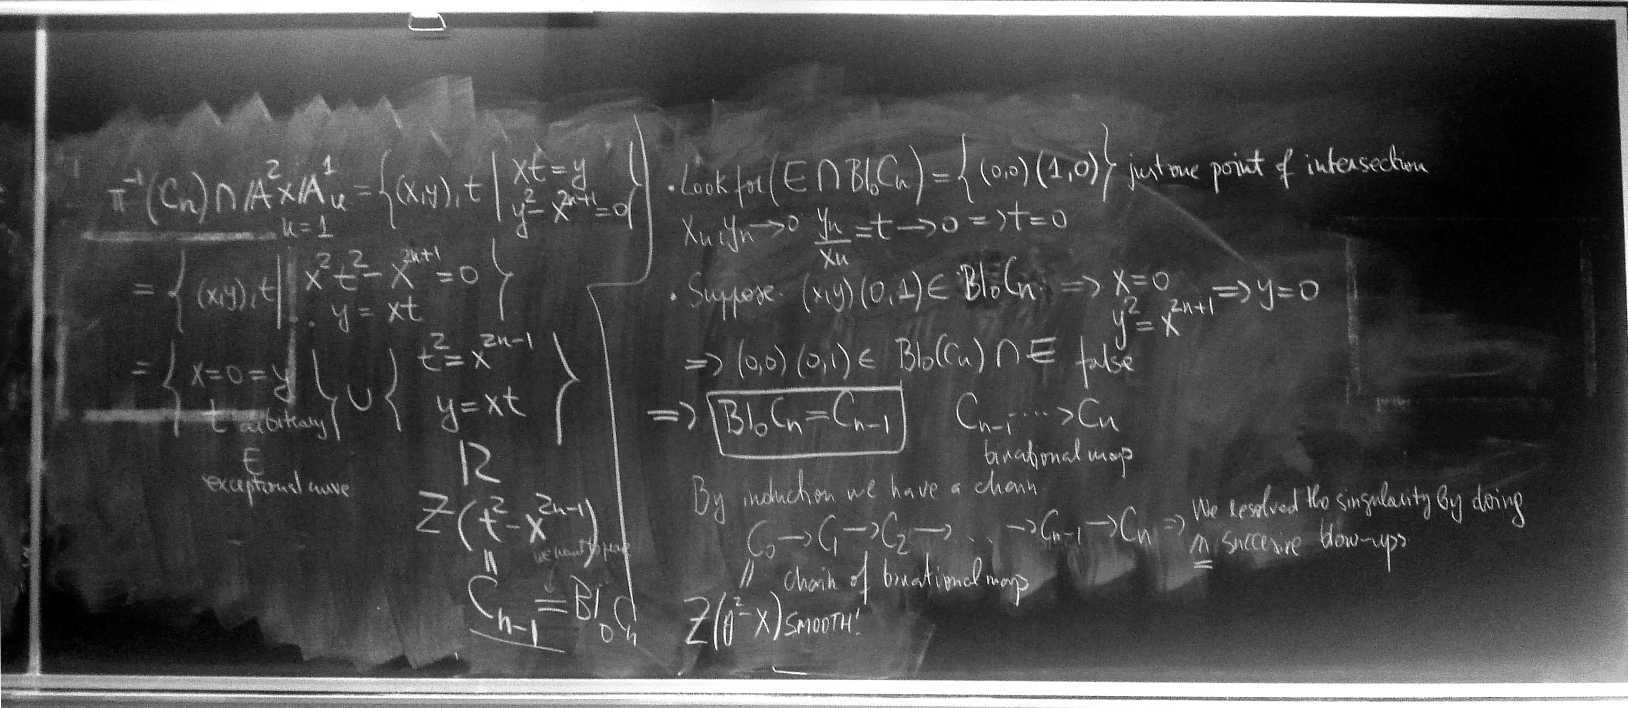
\includegraphics[width=1\textwidth]{2}

\textbf{Example: }Show that the blowup of $\mathbb{P}^{1}$ at one
point is isomorphic to the blowup of $\mathbb{P}^{2}$ in two points.

\textbf{Proof:} We have $\mathbb{P}^{1}\times\mathbb{P}^{1}\cong Q=\left(x_{0}x_{3}-x_{1}x_{2}\right)$
in $\mathbb{P}^{3}$. We blowup the ideal $\left(x_{0},x_{1},x_{2}\right)$
vanishing at $\left[0:0:0:1\right]$ to obtain
\[
\mbox{Bl}_{\left(x_{0},x_{1},x_{2}\right)}Q=\tilde{Q}\subseteq\mathbb{P}^{3}\times\mathbb{P}^{2}.
\]


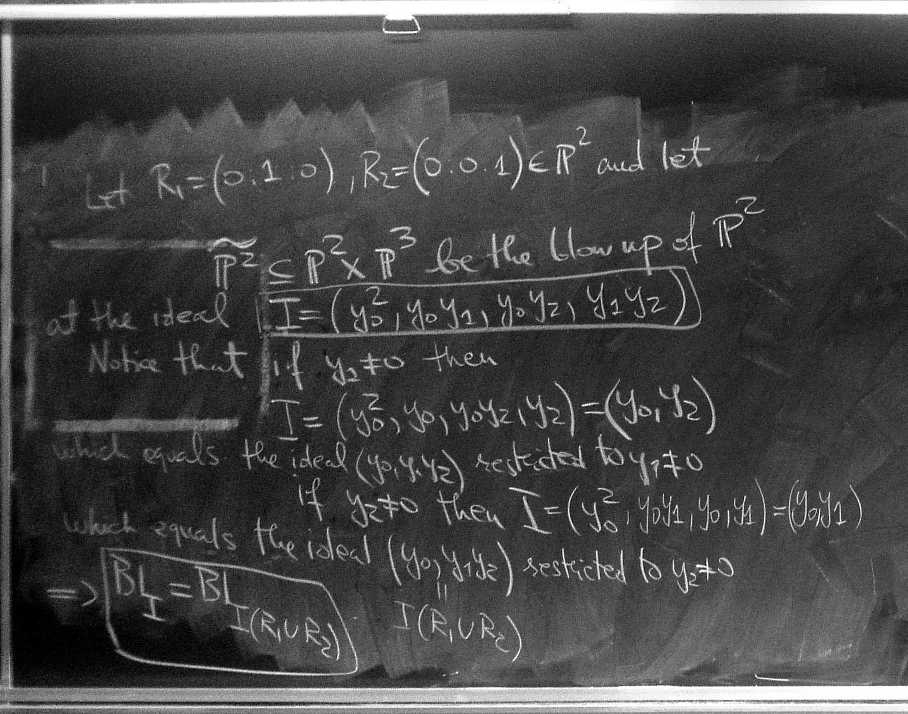
\includegraphics[height=0.27\paperheight]{4}~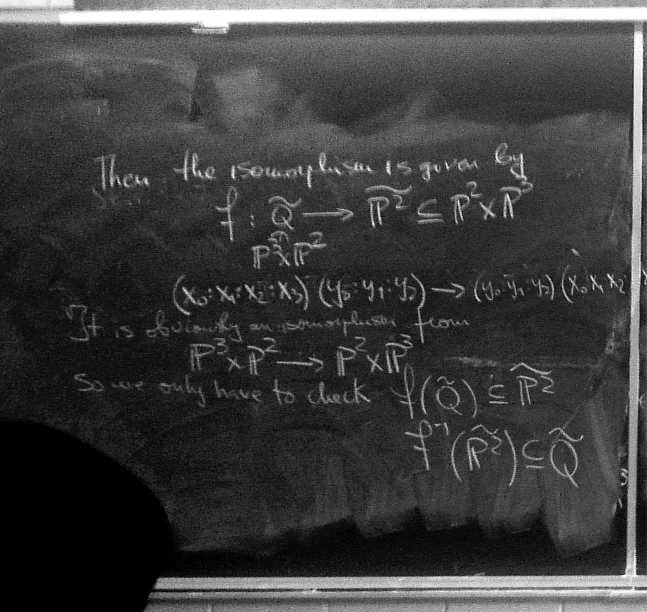
\includegraphics[height=0.27\paperheight]{5}

\textbf{\newpage{}}

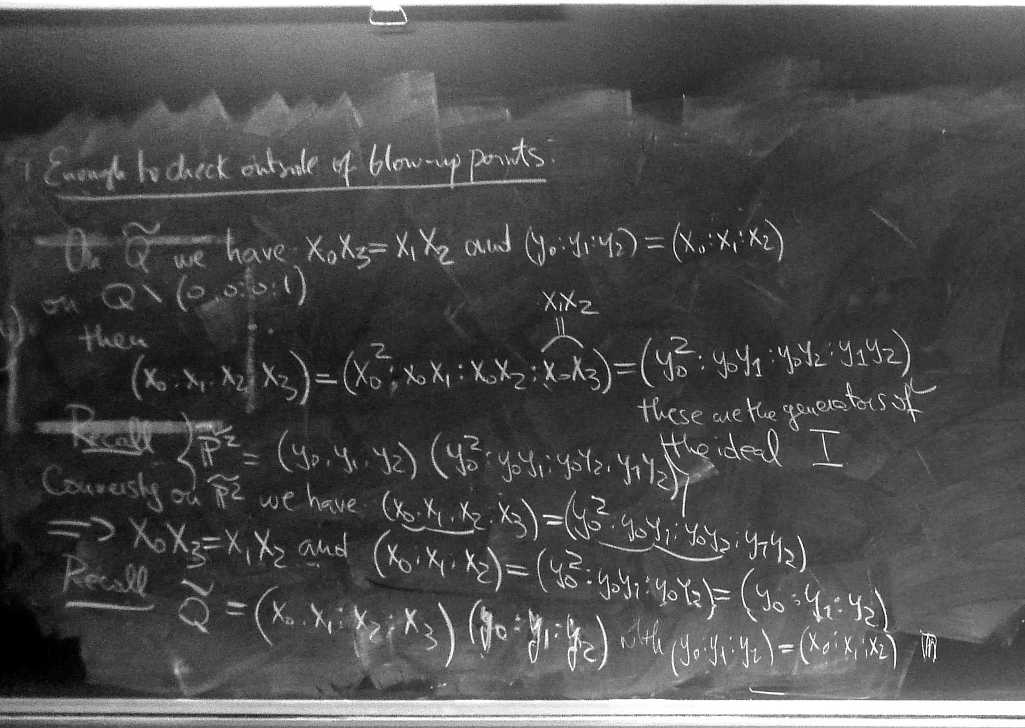
\includegraphics[height=0.27\paperheight]{6}~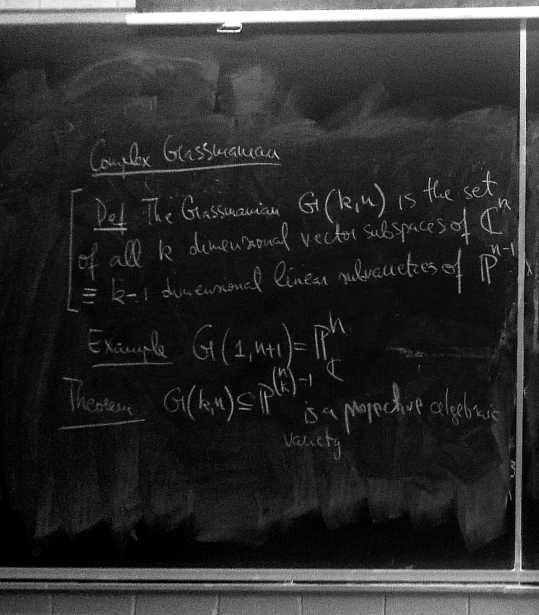
\includegraphics[height=0.27\paperheight]{7}

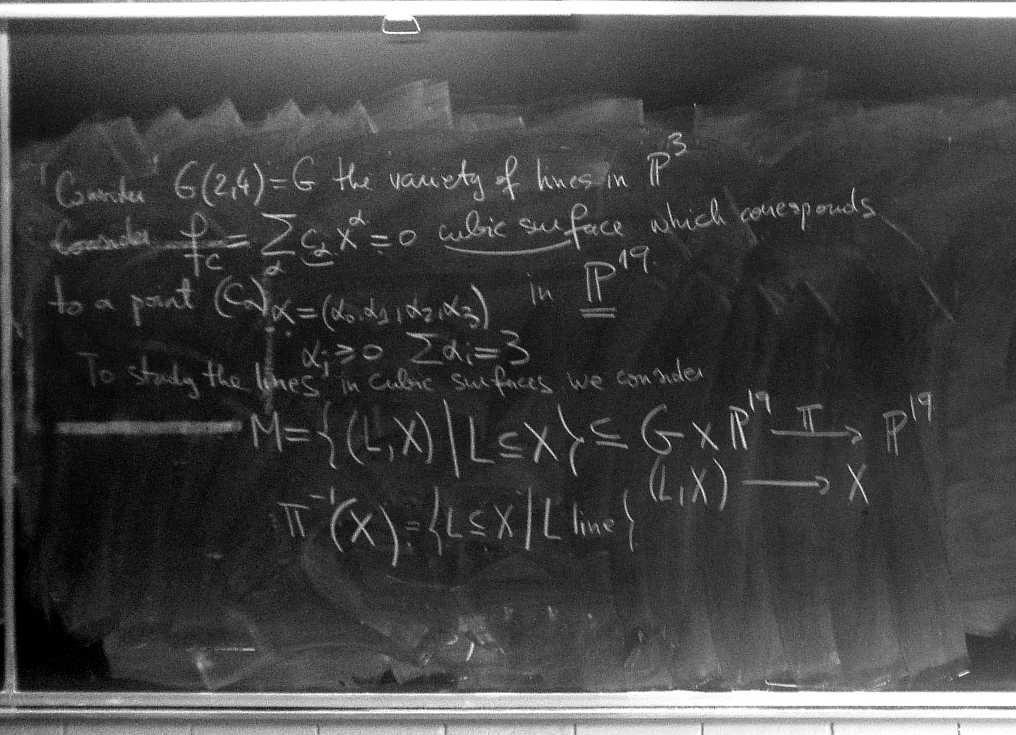
\includegraphics[height=0.27\paperheight]{8}

\textbf{Lemma:}
\begin{enumerate}
\item [a)]$M$ is a smooth 19-dimensional variety
\item [b)] The projection map $\pi:M\to\mathbb{P}^{19}$ is a local isomorphism
i.e. covering map
\[
\forall x\in\mathbb{P}^{19}\;\exists U_{x}\quad\pi^{-1}\left(U_{x}\right)=\coprod S_{i}
\]
 union of disjoint sets s.t. $S_{i}\to U_{x}$ homomorphism.
\end{enumerate}
In particular all fibers have the same cardinal $\left|\pi^{-1}\left(x\right)\right|$
constant finite.

The number of lines on a cubic smooth surface is independent of the
particular cubic chosen

(I have no idea what this is on about, looks like its in Gathmann
though)
\end{document}
